\documentclass[Analysis-3]{subfiles}
\usepackage{style}

\begin{document}
\chapter*{Lecture 24} %Set chapter name
\addcontentsline{toc}{chapter}{Lecture 24} %Set chapter title
\setcounter{chapter}{24} %Set chapter counter
\setcounter{section}{0}
\begin{Thm}{}{}\label{thm24:1}
    Let, $f: \mathcal{O}_n \to \R$ be a $C^1$ function and $\gamma$ be a piecewise smooth $C^1$ curve on $\mathcal{O}_n$, joining two points $A$ and $B$. Then
    \[\int_c \vec{\nabla}f\cdot d\vec{r} = f(B)-f(A)\]
    Which means the above line integral is "independent of parametrization".
\end{Thm}

\textit{Proof.} Let, $r$ be a parametrization of the curve $\gamma$ and $r :[a,b] \to \mathcal{O}_n$ uch that $r(a)=A$ and $r(b)=B$.

\begin{wrapfigure}{r}{0.25\textwidth}
    \centering
    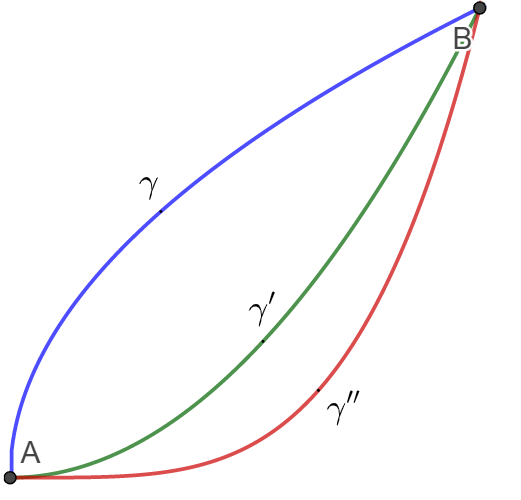
\includegraphics[width=.78\linewidth]{figures/lec-24.1.png}
    \caption{paths from A to B}
\end{wrapfigure}

Evaluating the LHS gives,
\begin{align*}
    \int_c \vec{\nabla}f\cdot d\vec{r} & \overset{\mathrm{(1)}}{=} \int_a^b \nabla f(r(t)) \cdot r'(t) dt \\
    &= \int_a^b \left(\sum_{i=1}^{n} \pdv{f}{r_i}\times r_i'(t) \right) dt \\
    &=\int_a^b \dv{t}(f(r(t))) dt\\
    &= f(r(b)) - f(r(a)) \\
    &= f(B) - f(A)
\end{align*}
\begin{center}
    (1) follows from \ref{eq:3}.
\end{center}


$\bullet$ This result has an important consequence that we often use in Physics. 

 "Workdone by a conservative force always depends on the \textcolor{violet}{starting point} and the \textcolor{violet}{end point}, not on the path followed by the particle." 
\vspace*{0.2cm}

$\bullet$ We know, if the force is conservative then we can define potential energy $U$ as $ \vec{F} = -\vec{\nabla }U$. Workdone by the force is simply the change of potential.

\vspace*{0.2cm}

Now we will recall the basics of the "Planes and Normals".

\vspace*{0.2cm}

\section{Planes and Normals}
Let, $\vec{P_0} = \langle x_0,y_0,z_0 \rangle$ be a fixed vector in $\R^3$. $\vec{N} = \langle a,b,c \rangle \neq \vec{0}$. The plane through $\vec{P_0}$ with $\vec{N}$ as normal to this plane is,
$$ := \{\vec{P_0} + \vec{P} | \vec{P}\cdot \vec{N} = 0\} = \{\vec{r} | (\vec{r}-\vec{P_0})\cdot \vec{N} = 0 \} $$

\underline{\textbf{Equation of the plane}:} Consider an  arbitary point $\vec{P} = \langle x,y,z\rangle$ on the plane then, $$\langle x-x_0,y-y_0,z-z_0\rangle \cdot \langle a,b,c \rangle = 0$$
So, equation of the plane is $a(x-x_0)+b(y-y_0) +c(z-z_0)= 0 \cdots \label{eq:4} (\ref{eq:4})$

  \vspace{1cm}

Let $\vec{Q_1},\vec{Q_2}$ be independent in $\R^3$ and also satisfying $\vec{Q_i} \cdot \vec{N} = 0$. clearly, $\vec{Q_1}\times \vec{Q_2} \neq \vec{0}$. We can see $(\vec{Q_1}\times \vec{Q_2}) \cdot \vec{Q_i} = 0$ .i.e $\{\vec{Q_1},\vec{Q_2},\vec{Q_1}\times \vec{Q_2}\}$ form a basis of $\R^3$. 

$$\therefore \hspace{0.2cm}\vec{Q_1}\times \vec{Q_2} = c \vec{N}$$
So, $\{\vec{P_0} + r_1 \vec{Q_1} + r_2 \vec{Q_2} | r_1,r_2 \in \R \}$ describes the same plane as \ref{eq:4}. 

\section{Surface and Surface Integrals}
\begin{Def}{Region}{}
    A subset $\mathcal{R} \subseteq \R^2$ is called a \enquote{Region} if $\mathcal{R}$ is Open ans $\mathcal{R}$ has an area (i.e. $\partial \mathcal{R}$ is \textbf{content zero})
\end{Def}

\begin{Def}{Parametrized Surface}{}\label{def:ps}
    $\mathcal{L}$et $\mathcal{R} \subseteq \R^2$ be a region. $\mathcal{A}$ $C^1$ function $r:\mathcal{R} \to \R^3$ said to be a \enquote{Parametrized Surface} if :
  \begin{itemize}
    \item The component functions $r_i$ have a bounded partials
    \item $r$ is $1-1$ function
    \item $\pdv{\vec{r}}{u} \times \pdv{\vec{r}}{v} \neq \vec{0}$ for all $(u,v) \in \R^2$. This menas total derivative of $r$ has rank $2$.
  \end{itemize}
 $\$$ We will call range of $r$ as a \textbf{Surface}, $ \mathcal{S} = \text{ran}(r)$.
\end{Def}



\end{document}